\section{Lecture 12}

Recall that we discussed the following iteration as part of gradient descent.
\[
    \mathbf{x}_{k+1} = \mathbf{x}_k - \alpha_k \cdot \nabla f(\mathbf{x}_k).
\]
For the remainder of this lecture, we assume that $f$ is twice continuously differentiable. 

\begin{defn}[Contraction]
    A function $f \colon \mathbb{R}^d \to \mathbb{R}^d$ is said to be a \emph{contraction} if 
    \[
        \norm{f(\mathbf{x}) - f(\mathbf{y})} \leq \alpha \cdot \norm{\mathbf{x} - \mathbf{y}}
    \]
    for all $\mathbf{x}, \mathbf{y} \in \mathbb{R}^d$, where $\alpha \in [0,1)$. If $\alpha = 1$, we say that $f$ is \emph{non-expansive}.
\end{defn}

\begin{defn}[Fixed Point]
    $\mathbf{x}^* \in \mathbb{R}^d$ is said to be a \emph{fixed point} of $g \colon \mathbb{R}^d \to \mathbb{R}^d$ if $g(\mathbf{x}^*) = \mathbf{x}^*$. 
\end{defn}

\begin{lem}[Banach Fixed Point Theorem]
    If $F \colon \mathbb{R}^d \to \mathbb{R}^d$ is a contraction, then $F$ admits a unique fixed point $\mathbf{x}^*$. Furthermore, the iteration $\mathbf{x}_{n+1} \vcentcolon= F(\mathbf{x}_n)$ converges to $\mathbf{x}^*$ exponentially starting from any arbitrary point $\mathbf{x}_0 \in \mathbb{R}^d$. 
\end{lem}
Note: The above holds more generally for $F \colon S \to S$ where $(S,d)$ is a complete metric space. 
\begin{proof}
    \textbf{Uniqueness.} If $\mathbf{x}$ and $\mathbf{y}$ are two fixed points of $F$, then we have $F(\mathbf{x}) = \mathbf{x}$ and $F(\mathbf{y}) = \mathbf{y}$. Thus, 
    \[
        \norm{\mathbf{x} - \mathbf{y}} = \norm{F(\mathbf{x}) - F(\mathbf{y})} \leq \alpha \cdot \norm{\mathbf{x} - \mathbf{y}}
    \]
    where $\alpha \in [0,1)$, which gives us $\mathbf{x} = \mathbf{y}$.

    \textbf{Existence.} Let $\mathbf{x}_{n+1} = F(\mathbf{x}_n)$ and $\mathbf{x}_{n+2} = F(\mathbf{x}_{n+1})$. We then have
    \begin{align*}
        \norm{\mathbf{x}_{n+2} - \mathbf{x}_{n+1}} &= \norm{F(\mathbf{x}_{n+1}) - F(\mathbf{x}_n)} \\
        &\leq \alpha \cdot \norm{\mathbf{x}_{n+1} - \mathbf{x}_n} \\
        &\leq \alpha^2 \cdot \norm{\mathbf{x}_n - \mathbf{x}_{n-1}} \\
        &\leq \alpha^{n+1} \cdot \norm{\mathbf{x}_1 - \mathbf{x}_0}
    \end{align*}
    As a result, we have
    \[
        \sum_{n=0}^{\infty} \norm{\mathbf{x}_{n+1} - \mathbf{x}_n} < \infty
    \]
    which gives us that $\{\mathbf{x}_n\}$ is Cauchy. Indeed, we have
    \begin{align*}
        \norm{\mathbf{x}_{n+m} - \mathbf{x}_n} &\leq \sum_{k=0}^{m-1} \norm{\mathbf{x}_{n+k-1} - \mathbf{x}_{n+k}} \\
        &\leq \sum_{k=0}^{m-1} \alpha^{k+n} \norm{\mathbf{x}_1 - \mathbf{x}_0} \\
        &= \alpha^n \cdot \frac{1-\alpha^m}{1-\alpha} \cdot \norm{\mathbf{x}_1 - \mathbf{x}_0} \\
        &\to 0 \quad \text{as } m,n \uparrow \infty.
    \end{align*}
    Thus, $\mathbf{x}_n \to \mathbf{x}^*$ for some $\mathbf{x}^*$. Further, we have $\mathbf{x}_{n+1} = F(\mathbf{x}_n)$. Letting $n \uparrow \infty$, we get $\mathbf{x}^* = F(\mathbf{x}^*)$ so that $\mathbf{x}^*$ is a fixed point of $F$. 
\end{proof}

We analyze a simple case where $f \colon \mathbb{R}^d \to \mathbb{R}^d$ is assumed to be twice continuously differentiable. Suppose that $\mathbf{x}^*$ is its (isolated) local minimum and $\nabla^2 f(\mathbf{x}^*) > 0$ (positive definite). We can find an $r > 0$ such that $\nabla^2 f(\mathbf{x}) > 0$ for all $\mathbf{x} \in \overline{B}_r(\mathbf{x}^*)$ by continuity. In particular, its eigenvalues are real and positive. Let $\lambda_{\min}(\mathbf{x})$ denote the least eigenvalue of $\nabla^2 f(\mathbf{x})$, and further, let $\lambda_0 \vcentcolon= \min_{\mathbf{x} \in \overline{B}_r(\mathbf{x}^*)} \lambda_{\min}(\mathbf{x})$. Let $\alpha \in (0,\lambda_0)$ and consider the gradient descent scheme with $\alpha_n \equiv \alpha$. Suppose $\mathbf{x}_{n_0} \in \overline{B}_r(\mathbf{x}^*)$. Since $\nabla f(\mathbf{x}^*) = \mathbf{0}$, Taylor's formula for $n \geq n_0$ gives us
\begin{align*}
    \mathbf{x}_{n+1} - \mathbf{x}^* &= \mathbf{x}_n - \mathbf{x}^* - \alpha \left( \nabla f(\mathbf{x}_n) - \nabla f(\mathbf{x}^*) \right) \\
    &= \left( \mathbf{I} - a \nabla^2 f(\Tilde{\mathbf{x}}_n) \right) \cdot (\mathbf{x}_n -\mathbf{x}^*) \quad \text{for some } \Tilde{\mathbf{x}}_n \in \overline{B}_r(\mathbf{x}^*) 
\end{align*}
Thus, 
\begin{align*}
    \norm{\mathbf{x}_{n+1} - \mathbf{x}^*} &\leq \norm{\mathbf{I} - a \nabla^2 f(\Tilde{\mathbf{x}}_n} \norm{\mathbf{x}_n -\mathbf{x}^*} \\
    &\leq (1 - a\lambda_{\min}(\Tilde{\mathbf{x}}_n)) \norm{\mathbf{x}_n -\mathbf{x}^*} \\
    &\leq (1 - a\lambda_0)  \norm{\mathbf{x}_n -\mathbf{x}^*}
\end{align*}
where $(1-a\lambda_0) \in (0,1)$. Thus, 
\[
     \norm{\mathbf{x}_n -\mathbf{x}^*} = (1-a\lambda_0)^{n-n_0}  \norm{\mathbf{x}_{n_0+1} -\mathbf{x}^*} \to 0
\]
If we use general step sizes $\{\alpha_n\}$ instead of the constant step size, a similar argument gives us
\[
     \norm{\mathbf{x}_n -\mathbf{x}^*} = e^{-\lambda_0 \sum_{m=n_0+1}^{\infty} \alpha_m}  \norm{\mathbf{x}_{n_0+1} -\mathbf{x}^*} \to 0.
\] 

Gradient descent is extremely popular since it is quite a simple scheme - however, it is not without its drawbacks. For example, the iterate may get stuck in a `shallow' local minimum and fail to reach the global minimum. The scheme also slows down considerably when it approaches local minima since the gradient magnitude becomes smaller and smaller. The biggest drawback is its performance on `pinched' landscaped where neighborhoods of local minima rise away extremely slowly in some directions, and extremely rapidly in other directions. An example of such a landscape is shown below in Figure \ref{fig:pinched}. 

\begin{figure}[!ht]
    \centering
    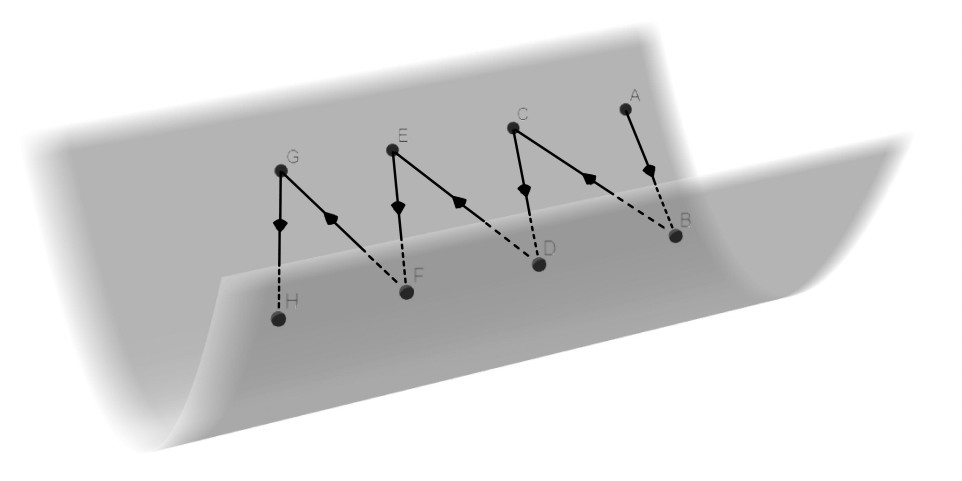
\includegraphics[width=0.7\linewidth]{pinched.png}
    \caption{A pinched landscape}
    \label{fig:pinched}
\end{figure}

As shown, gradient descent often `zigzags' along the alley rather than just moving down along it. 

\subsection*{Momentum Methods}

An easy fix for this is via the \textbf{momentum method}. To each iteration, we add a term proportional to the previous move, so that our iteration becomes
\[
    \mathbf{x}_{n+1} = \mathbf{x}_n - \alpha_n \cdot \nabla f(\mathbf{x}_n) + \beta_n (\mathbf{x}_n - \mathbf{x}_{n-1}).
\]
Usually, $\beta_n < \alpha_n$. For simplicity, we let $\alpha_n \equiv \alpha$ and $\beta_n \equiv \beta$. Setting $\mathbf{y}_n = \mathbf{x}_n - \mathbf{x}_{n-1}$, the iteration can be viewed of the following set of differential equations. 
\begin{align*}
    \dot{\mathbf{x}}(t) &= \mathbf{y}(t) \\
    \dot{\mathbf{y}}(t) &= -a \mathbf{y}(t) - \nabla f(\mathbf{x}(t))
\end{align*}
where $a \vcentcolon= (1 - \alpha/\beta) > 0$. This can be interpreted as Newtonian dynamics in a potential field $f$ with damping. A common example is a ball rolling down a rough hill. Thanks to its momentum, the ball is able to escape any points of local maxima, saddle points, inflection points, and even shallow local minima. It also does a better job of moving along a `flat' landscape than gradient descent. It quickly approaches the bottom of valleys where it eventually settles down, much faster than gradient dynamics. The iterate also locally oscillates dissipating energy before it settles down. 

\medskip 

Finally, note that we never evaluate the gradient analytically, but rather, it is approximated via one of the following schemes.
\begin{align*}
    \frac{\partial f}{\partial x_i}(\mathbf{x}) &\approx \frac{f(\mathbf{x} + \delta \mathbf{e}_i) - f(\mathbf{x})}{\delta} \\
    \frac{\partial f}{\partial x_i}(\mathbf{x}) &\approx \frac{f(\mathbf{x} + \delta \mathbf{e}_i) - f(\mathbf{x} - \delta \mathbf{e}_i)}{2\delta}
\end{align*}
The former requires only $d+1$ function evaluations while having a higher error of $\mathcal{O}(\delta)$. The latter requires $2d$ function evaluations but has a smaller error of $\mathcal{O}(\delta^2)$. 